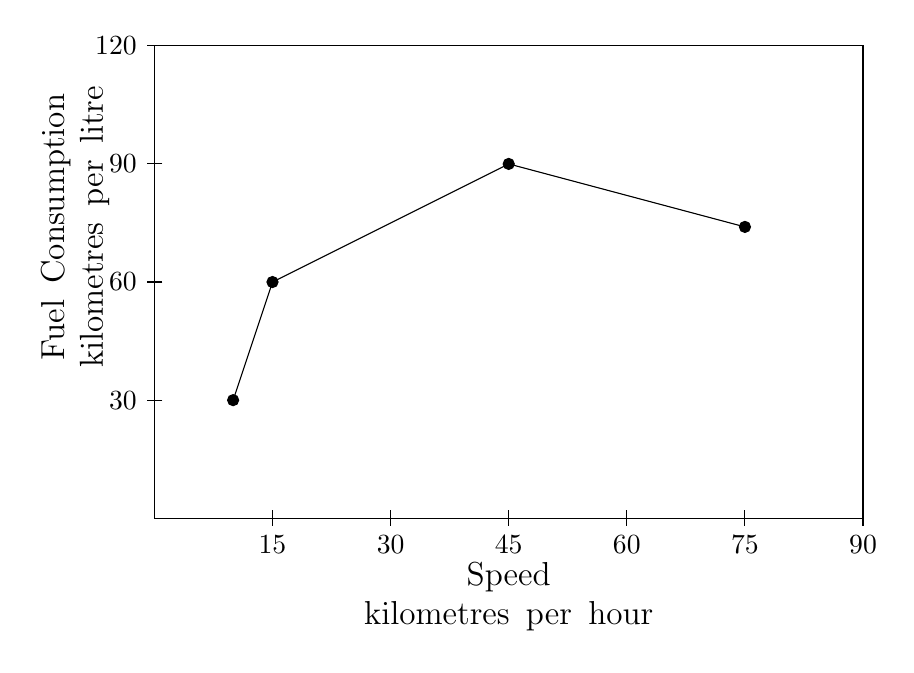
\begin{tikzpicture}
    \draw (0,6) rectangle (9,0);
    \node[font=\large] at (4.5,-1) {\begin{tabular}{c}
        Speed\\
     \brak{kilometres \,per\, hour}
    \end{tabular}};
    \node[font=\large, rotate=90] at (-1,3.7) {\begin{tabular}{c}
    Fuel \,Consumption \\
    \brak{kilometres \,per\, litre}\end{tabular}};

    \draw (1.5,0.1) -- (1.5,-0.1) node[below] {15};
    \draw (3,0.1) -- (3,-0.1) node[below] {30};
    \draw (4.5,0.1) -- (4.5,-0.1) node[below] {45};
    \draw (6,0.1) -- (6,-0.1) node[below] {60};
    \draw (7.5,0.1) -- (7.5,-0.1) node[below] {75};
    \draw (9,0.1) -- (9,-0.1) node[below] {90};

    \draw (0.1,1.5) -- (-0.1,1.5) node[left] {30};
    \draw (0.1,3) -- (-0.1,3) node[left] {60};
    \draw (0.1,4.5) -- (-0.1,4.5) node[left] {90};
    \draw (0.1,6) -- (-0.1,6) node[left] {120};

    \foreach \x/\y in {1/1.5, 1.5/3, 4.5/4.5,7.5/3.7}
        \filldraw (\x,\y) circle (2pt);

    \draw (1,1.5) --(1.5,3)-- (4.5,4.5) -- (7.5,3.7);
\end{tikzpicture}

